\section{Nonogram puzzle solver}

\renewcommand{\CURPATH}{puzzles/nonogram}

This is a sample one, from Wikipedia:

\begin{figure}[H]
\centering
\frame{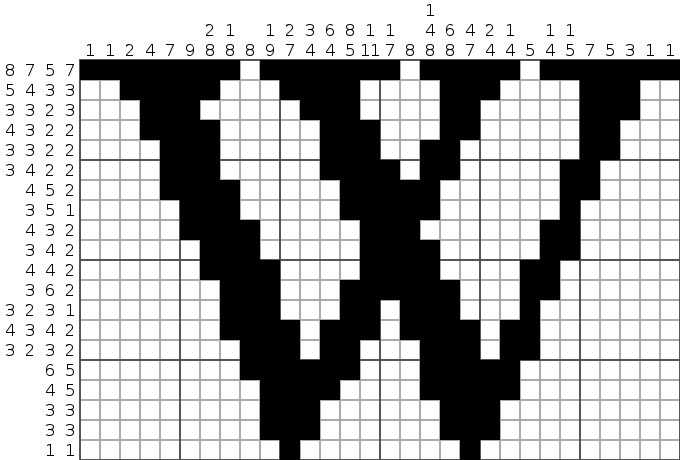
\includegraphics[scale=0.7]{\CURPATH/680px-Nonogram_wiki.png}}
\end{figure}

\lstinputlisting[style=custompy]{\CURPATH/nonogram_solver.py}

The result:

\begin{lstlisting}
sat                                                                                                       
******** ******* ***** *******
  *****   ****    ***    ***
   ***     ***    **     ***
   ****     ***   **     **
    ***     ***  **      **
    ***     **** **     **
    ****     *****      **
     ***     *****      *
     ****     ***      **
      ***     ****     **
      ****    ****    **
       ***   ******   **
       ***   ** ***   *
       **** *** **** **
        *** **   *** **
        ******   *****
         ****    *****
         ***      ***
         ***      ***
          *        *
\end{lstlisting}

How it works (briefly).
Given a row of width 8 and input (or \emph{clue}) like [3,2], we create two \emph{islands} of two bitstrings of corresponding
lengths:

\begin{lstlisting}
00000111
00000011
\end{lstlisting}

The whole length of each bitvector/bitstring is 8 (width of row).

We then define another variable: \verb|island_shift|, for each \emph{island}, which defines a count, on which a bitstring is shifted left.
We also calculate limits for each \emph{island}: position of each one must not be lower/equal then the position of the previous
\emph{island}.

All islands are then merged into one (\verb|merged_islands[]|) using OR operation:

\begin{lstlisting}
11100000
00001100

->

11101100
\end{lstlisting}

\verb|merged_islands[]| is a final representation of row --- how it will be printed.

Now repeat this all for all rows and all columns.

The final step: make corresponding bits in \verb|XXX_merged_islands[]| of each row and column to be equal to each other.
In other words, \verb|col_merged_islands[]| must be equal to \verb|row_merged_islands[]|, but rotated by 90°.

The solver is surprisingly fast even on hard puzzles.

Further work: colored nonograms.

